\section{Resultat}
Denna del av dokumentet presenterar resultatet av vårt arbete.
Här kommer beskrivs både hur systemet ser ut och används, samt hur det är uppbyggt rent tekniskt. Vidare beskrivs också hur utvecklingen inom gruppen fungerat.

\subsection{Översikt av systemet}
Det finns två huvuddelar i systemet. Handböckerna och kartoteket.

Handböckerna beskriver hur man förbereder olika typer av operationer.
Varje handbok har en lista med artiklar som behövs till operationen, en så kallad plocklista.
Artiklarna är kopplade till kartoteket, som bland annat innehåller information om var i förråden artiklarna finns placerade.

När en patient registreras skapas en instans av en handbok.
I denna instans kan man checka av en lista med artiklar som ska användas under operationen och även andra förberedelser.
En sammordnare kan se en översikt på hur långt man har kommit med de förberedelserna för varje instans.

I kartoteket finns information om alla artiklar som Region Östergötland har i förråden.
Här finns bland annat information om var artiklarna är placerade samt information relaterade till inköp av artiklar.

Systemet har två olika roller. Dessa är vanliga användare och administratörer. En administratör har rättigheter att skapa, redigera och publicera handböcker. De har också rättighet att redigera kartoteket. En administratör kan på så vis ses som en sammordnare av operationer. En vanlig användare kan ses som en sjuksköterska som förbereder operationer. Det finns i systemet funktionalitet för att skapa användare med administratörsrättigheter.

\subsection{Tekniker}
Här beskrivs vilka tekniker som ligger bakom systemet.

\subsubsection{Översikt}
Programmet är uppdelat i två delar, en serverdel och en klientdel. I figur \ref{fig:overview} visas en översikt av systemet.

\begin{figure}[htbp]
  \centering
  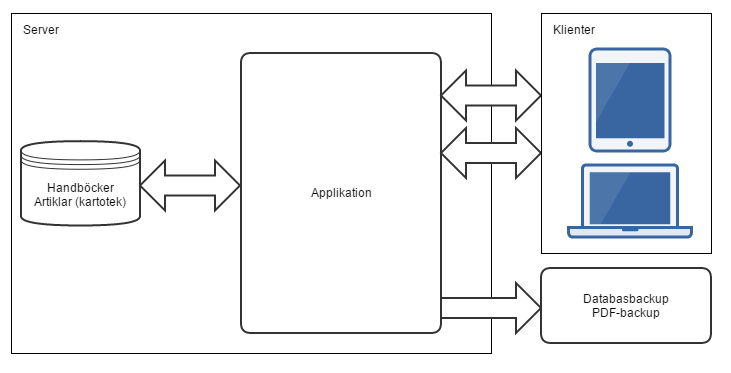
\includegraphics[width=0.9\textwidth]{images/overview.png}
  \caption{Översikt av systemet}
  \label{fig:overview}
\end{figure}
Serverdelen består av databaskopplingar som kopplas ihop och distribueras ut genom hemsidor till klienterna. Servern kan köras i en Windowsmiljö. Hemsidan är responsiv och fungerar på surfplattor och datorer i olika format.


I figur \ref{fig:techoverview} kan man se en översikt över de mest betydelsefulla tekniker och bibliotek som används för att bygga upp programmet.
\begin{figure}
  \centering
  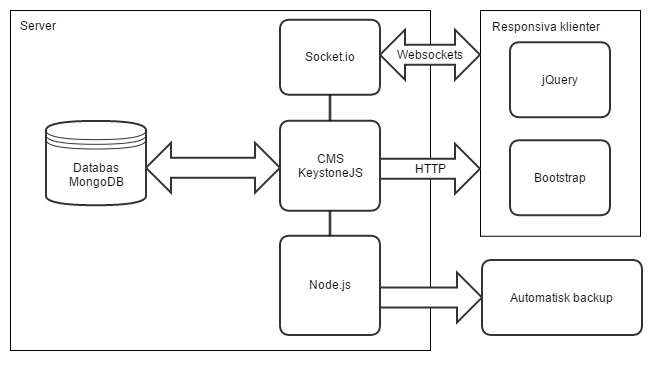
\includegraphics[width=0.9\textwidth]{images/techoverview.png}
  \caption{En översikt över tekniken}
  \label{fig:techoverview}
\end{figure}
\subsubsection{Back-end}
Koden till servern har skrivits helt i javascript.
Grunden till programmet är node.js vilket är en plattform för att utveckla självständiga program i javascript med inbyggd pakethanterare.

Det största och mest betydelsefulla ramverket för detta projekt är KeystoneJS, ett CMS-ramverk till node.js.

För realtidskommunikation används ett programmeringsinterface vid namn Socket.IO \cite{socketio}.
Socket.IO väljer automatiskt hur datan ska skickas beroende på vilken webbläsare som används och vad den stödjer.
Socket.io är event-baserat vilket betyder att man skapar events på antingen klient eller serversida som man sedan kan trigga från motsatt sida.
Vanliga javascript-object kan skickas tillsammans med eventen.

\subsubsection{Front-end}
På klientsidan används bootstrap\cite{bootstrap}, jQuery\cite{jquery} och LESS \cite{less}.

\subsubsection{Struktur}
Varje enskild sida har minst en skriptfil, en css fil och en html fil. På de sidor där det blivigt stora skripts så har skriptfilen delats upp i flera filer.

\subsubsection{Säkerhetskopiering och reservsystem}
Det ställs stora krav på att handböckerna alltid ska finnas tillgängliga då de ska användas på ett sjukhus där ett fel kan få stora konsekvenser. Detta innebär att ett reservsystem måste finnas till hands ifall systemet slutar fungera. Detta har lösts genom ett system där pdf-kopior av handböcker skapas. Handböckerna hamnar i en mapp-struktur där de sorteras på specialitet och operation. Kopian sparas med ett versionnummer, vilket gör att kopior av gamla versioner av operationer fortfarande finns kvar och kan skrivas ut. Var denna mapp-strukturen ska hamna bestäms i en konfigurationsfil.
Kopiorna skapas genom att en funktion, som kollar igenom alla handböcker för att se om har uppdaterats sedan senaste kopieringen, körs med ett givet tidsintervall som ställs in i konfigurationsfilen. Om en operation har uppdaterats så körs en funktion som använder en modul, som heter wkhtmltopdf, för att kalla på ett program som också heter wkhtmltopdf. Wkhtmltopdf använder en osynlig webbläsare för att skapa en pdf-kopia. Hur kopiorna ser ut kan ses i figur \ref{fig:pdf-start} och figur \ref{fig:pdf-end}. Utseendet ändras genom att speciell css för utskrift finns och wkhtmltopdf körs med utskrift som mediatyp.  

\begin{figure}
  \centering
  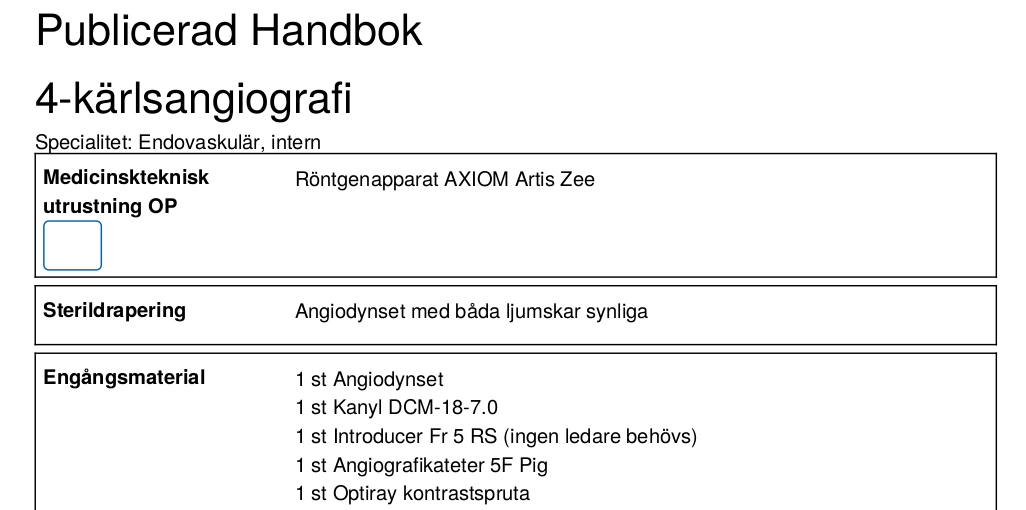
\includegraphics[width=0.9\textwidth]{images/pdf-start.png}
  \caption{Början på en pdf-kopia.}
  \label{fig:pdf-start}
\end{figure}

\begin{figure}
  \centering
  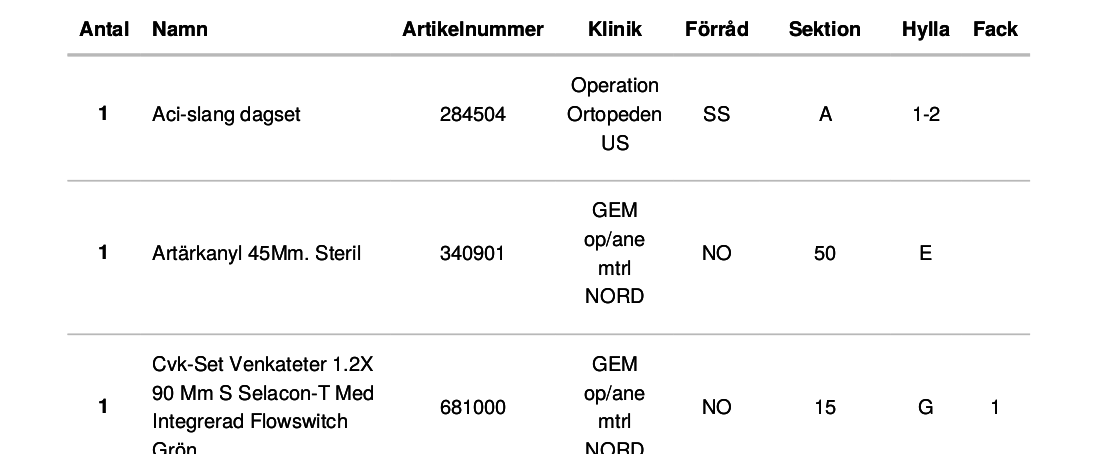
\includegraphics[width=0.9\textwidth]{images/pdf-end.png}
  \caption{Plocklista i en pdf-kopia.}
  \label{fig:pdf-end}
\end{figure}

Säkerhetskopiering av databasen finns implementerat. Det finns ett tidsintervall som går att ställa in i konfigurationsfilen så körs en funktion som använder en modul som heter mongo-utils för att kalla på mongodump som tar en kopia på databasen och lägger den i en mapp med dagens datum. 

\subsection{Funktionalitet}
Här beskrivs syftet och funktionalitet hos olika delar av produkten.

\subsubsection{Översiktsvy}
Som tidigare nämnts finns en översiktsvy över alla operationsförberedelser.
Denna sida visar alla operationsförberedelser och hur långt de är fortskridna, alltså hur många procent av förberedelserna och artiklarna som checkats av.
Här används Socket.IO för att hela tiden hålla information uppdaterad.

\begin{figure}[h!]
  \centering
  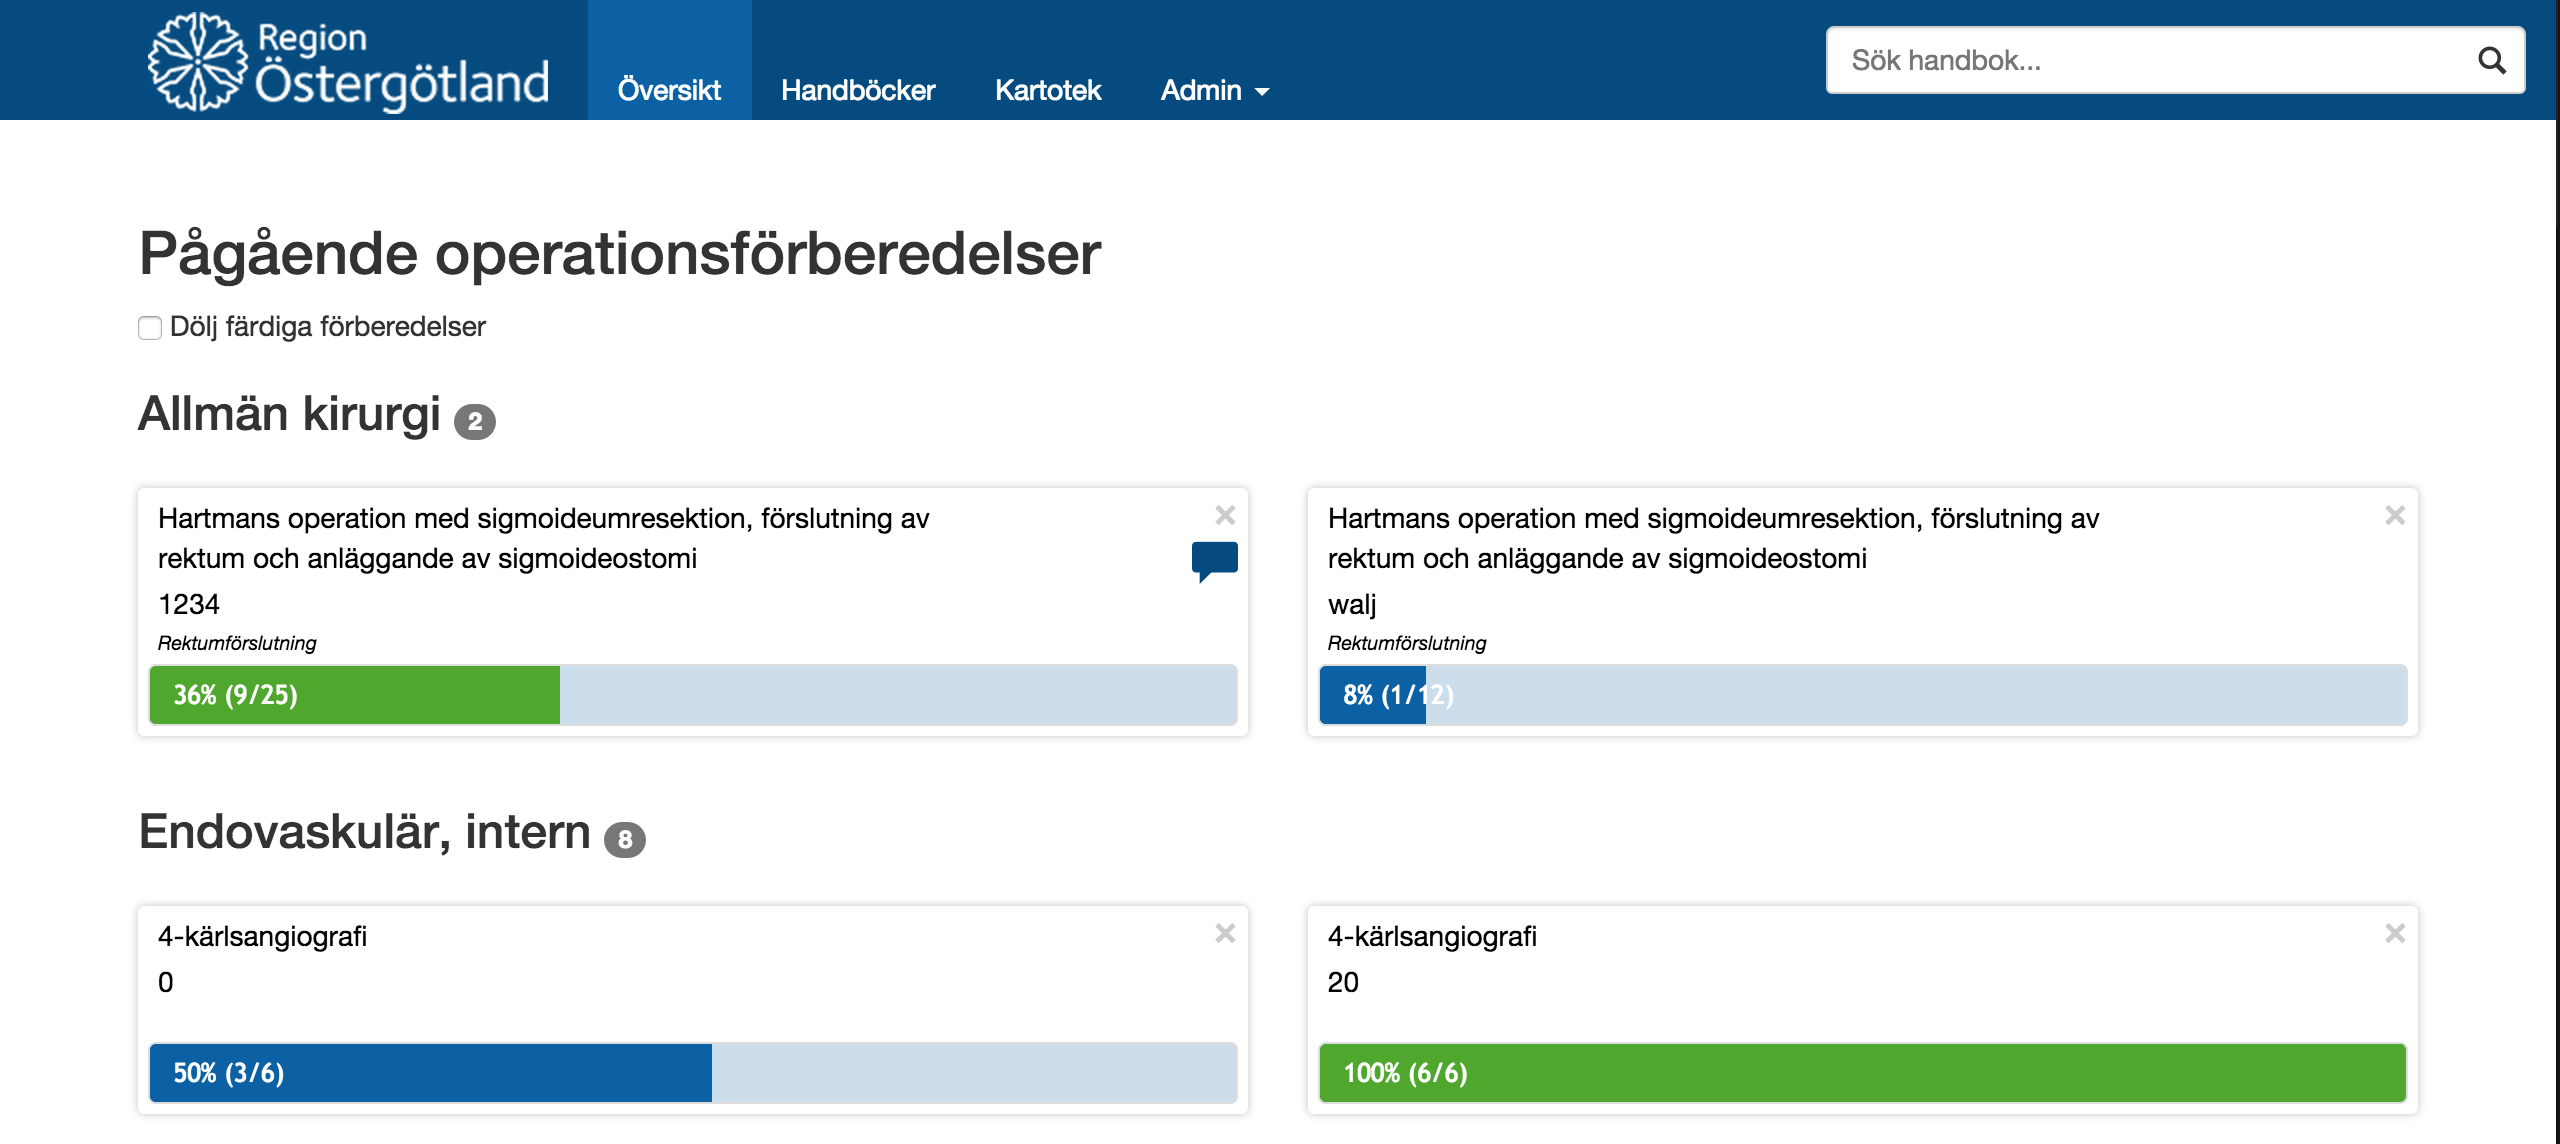
\includegraphics[width=0.95\textwidth]{images/site/overview.png}
  \caption{Bild på översiktsvyn}
  \label{fig:siteoverview}
\end{figure}

I figur \ref{fig:siteoverview} kan man se hur förberedelserna är kategoriserade beroende på vilken kirurgisk specialitet handboken tillhör.
Ibland är det olika samordnare beronde på specialitet och det är då enkelt för en samordnare att hitta de operationerna som personen är ansvarig över.
En ikon för kommentarer dyker upp om någon valt att kommentera en artikel. En samordnade kan då klicka på kommentarsikonen för att att få upp en lista över dessa kommentarer.

\subsubsection{Handbok}
En handbok innehåller information om en operationsförberedelse. All information i en handbok är uppdelad i olika rubriker. Dessa rubriker är i sin tur uppdelade i olika processer.
I figur \ref{fig:handbok} ser man dels de olika processerna (Preoparea, anestesi, allmänt och operation) samt rubrikerna som hör till processen Anestesi (Övrigt, premedicinering, blodrekvisition och  antibiotika).

\begin{figure}[h!]
  \centering
  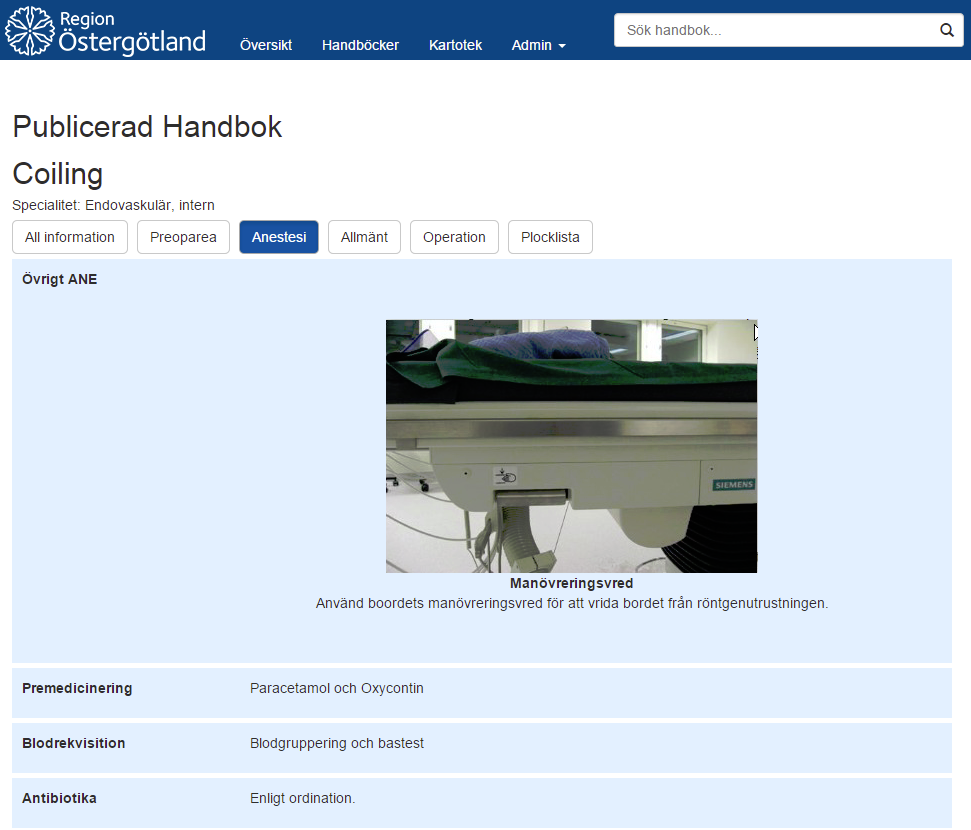
\includegraphics[width=0.9\textwidth]{images/site/handbok.png}
  \caption{En handbok}
  \label{fig:handbok}
\end{figure}

Man kan även se att handböckerna har stöd för bilder.

\subsubsection{Sökfunktion}
Ett krav är att det ska vara lätt att hitta en handbok.
Därför kan man söka både på operationens namn men även på alternativa sökord (taggar), dessa är bra att ha då de medicinska termerna ibland kan vara svåra att komma ihåg.
I figur \ref{fig:search} kan man se sökresultaten där namnet på operationen står i större storlek, och sökorden kursivt i mindre storlek.

\begin{figure}[h!]
  \centering
  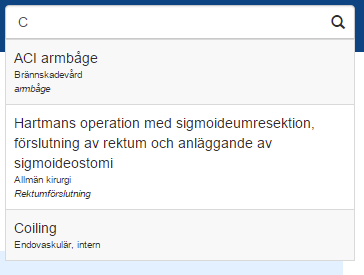
\includegraphics[width=0.5\textwidth]{images/site/search}
  \caption{Sökfunktionen}
  \label{fig:search}
\end{figure}


\subsubsection{Lista med handböcker}
Applikationen innehåller en enkel lista med alla handböcker. En vanlig användare kan se handböcker som är publicerade medan en administratör också kan se handböcker i tillstånden utkast, redigering och granskning. %Note to self(Daniel):Kan en handbok vara i redigering?
Listan går att sortera på valfri kolumn och kan även grupperas beroende på vilken specialitet handboken tillhör.
Se figur \ref{fig:list} för ett exempel.

\begin{figure}[h!]
  \centering
  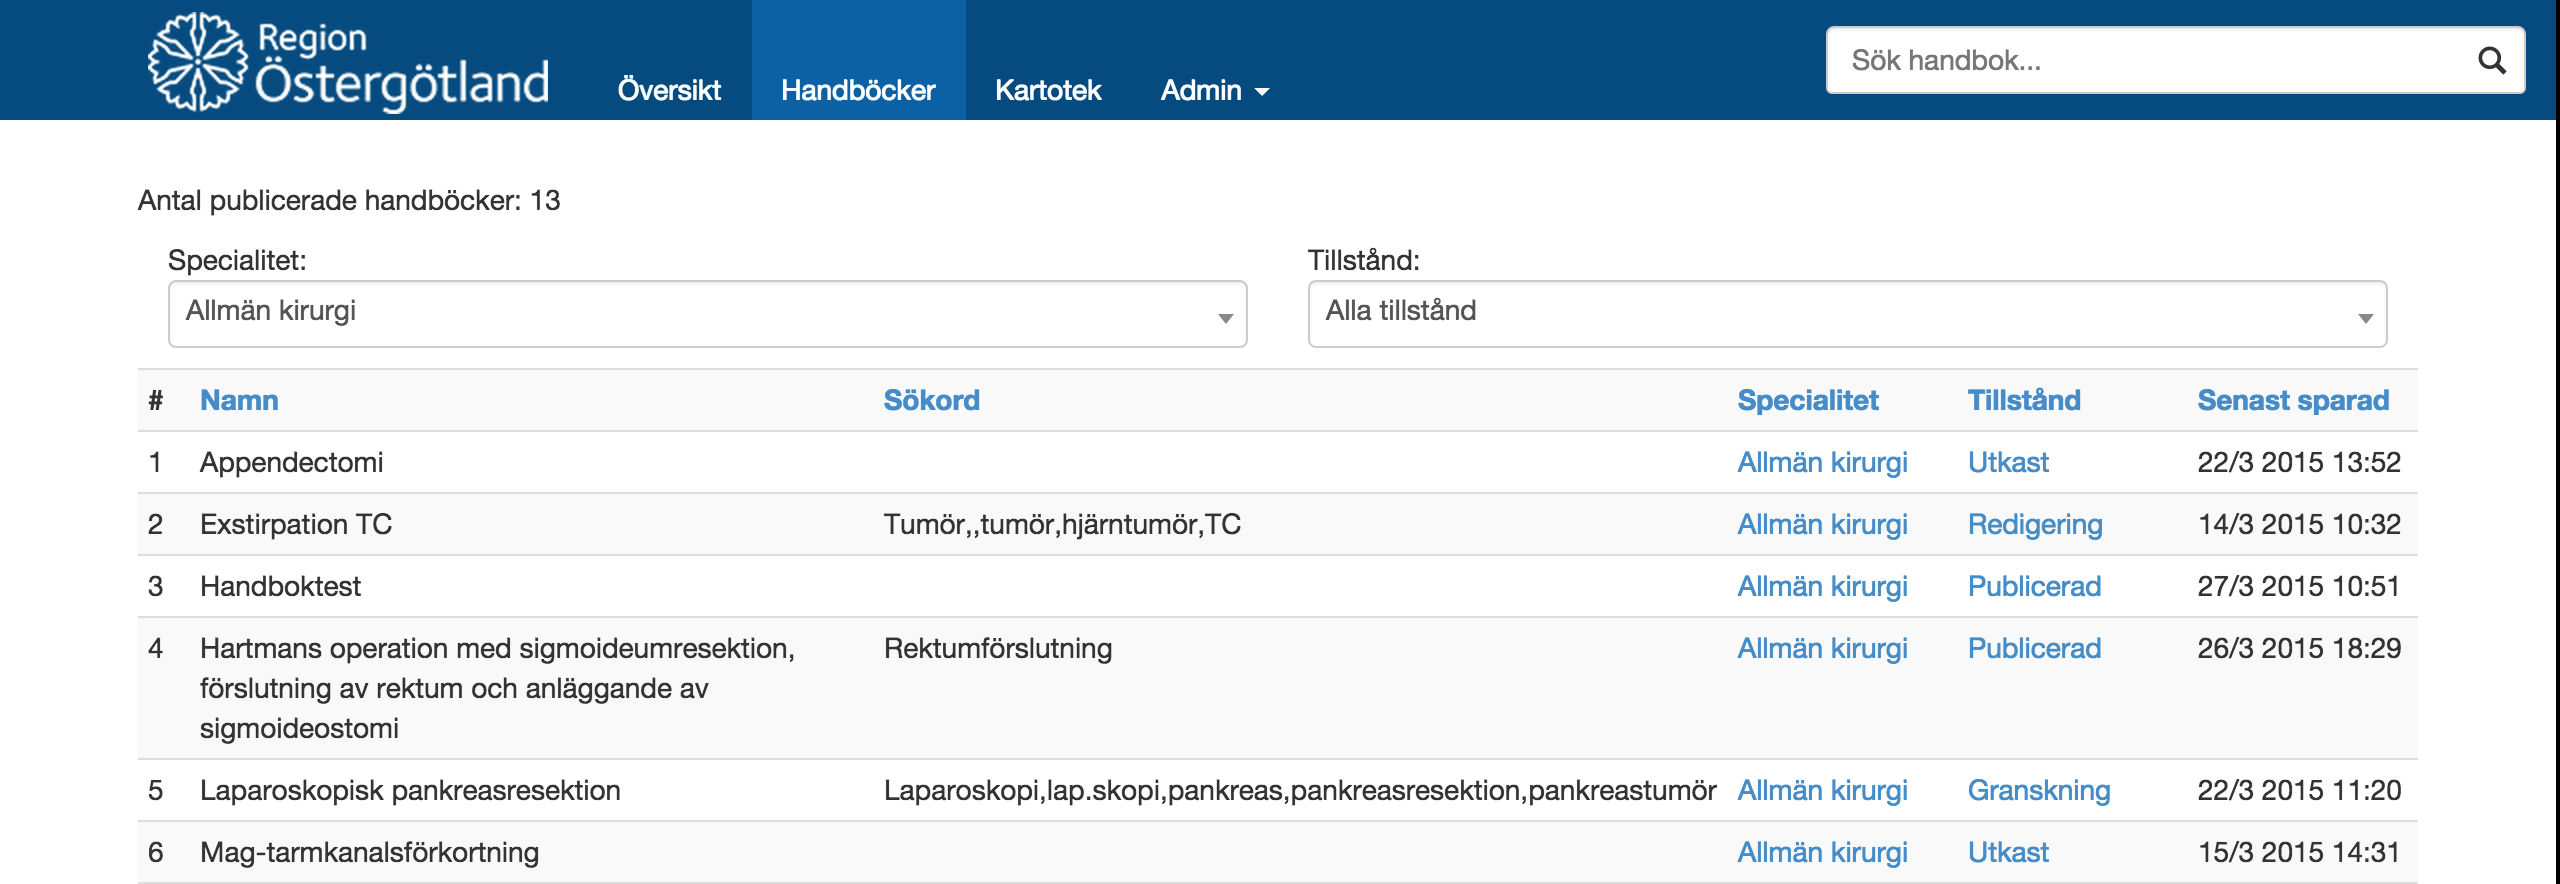
\includegraphics[width=0.95\textwidth]{images/site/list}
  \caption{Lista med handböcker}
  \label{fig:list}
\end{figure}

\subsubsection{Tillstånd}
Flödet för att skapa en handbok involverar flera steg och en handbok kan befinna sig i olika tillstånd.
Se figur \ref{fig:model} för en övervy.

\begin{figure}[h!]
  \centering
  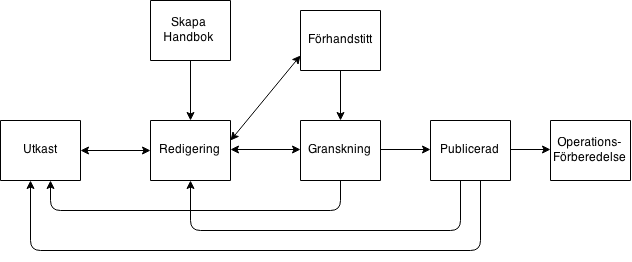
\includegraphics[width=0.7\textwidth]{images/model}
  \caption{Handböcker och deras olika tillstånd}
  \label{fig:model}
\end{figure}

När man först vill skapa en handbok så hamnar man i ett redigeringsläge,
där man kan lägga till information om handboken, som artiklar i plocklista,
beskrivning av operationen.
Härifrån kan man välja att förhandsgranska, för att se om den ser ok ut,
eller skicka till granskning, där den går vidare till publicering
efter någon annan läst igenom materialet och de tycker det ser rätt ut.
Om man har en handbok i redigeringsläge som inte är klar så hamnar den även i
''utkast''-läge, likt en email-system.
Slutligen kan en publicerad handbok gå vidare till att bli en
operationsförberedelse om det är dags att utföra en sådan operation
som beskrivs i handboken.

\subsubsection{Redigering}
I redigeringsvyn skapar man innehållet i en handbok. Det går bland annat lägga till synonymer, processteg med tillhörande information och artiklar från kartoteket. I figur \ref{fig:handboksredigering} visas ett exempel på hur denna redigering ser ut. 

\begin{figure}[h!]
  \centering
  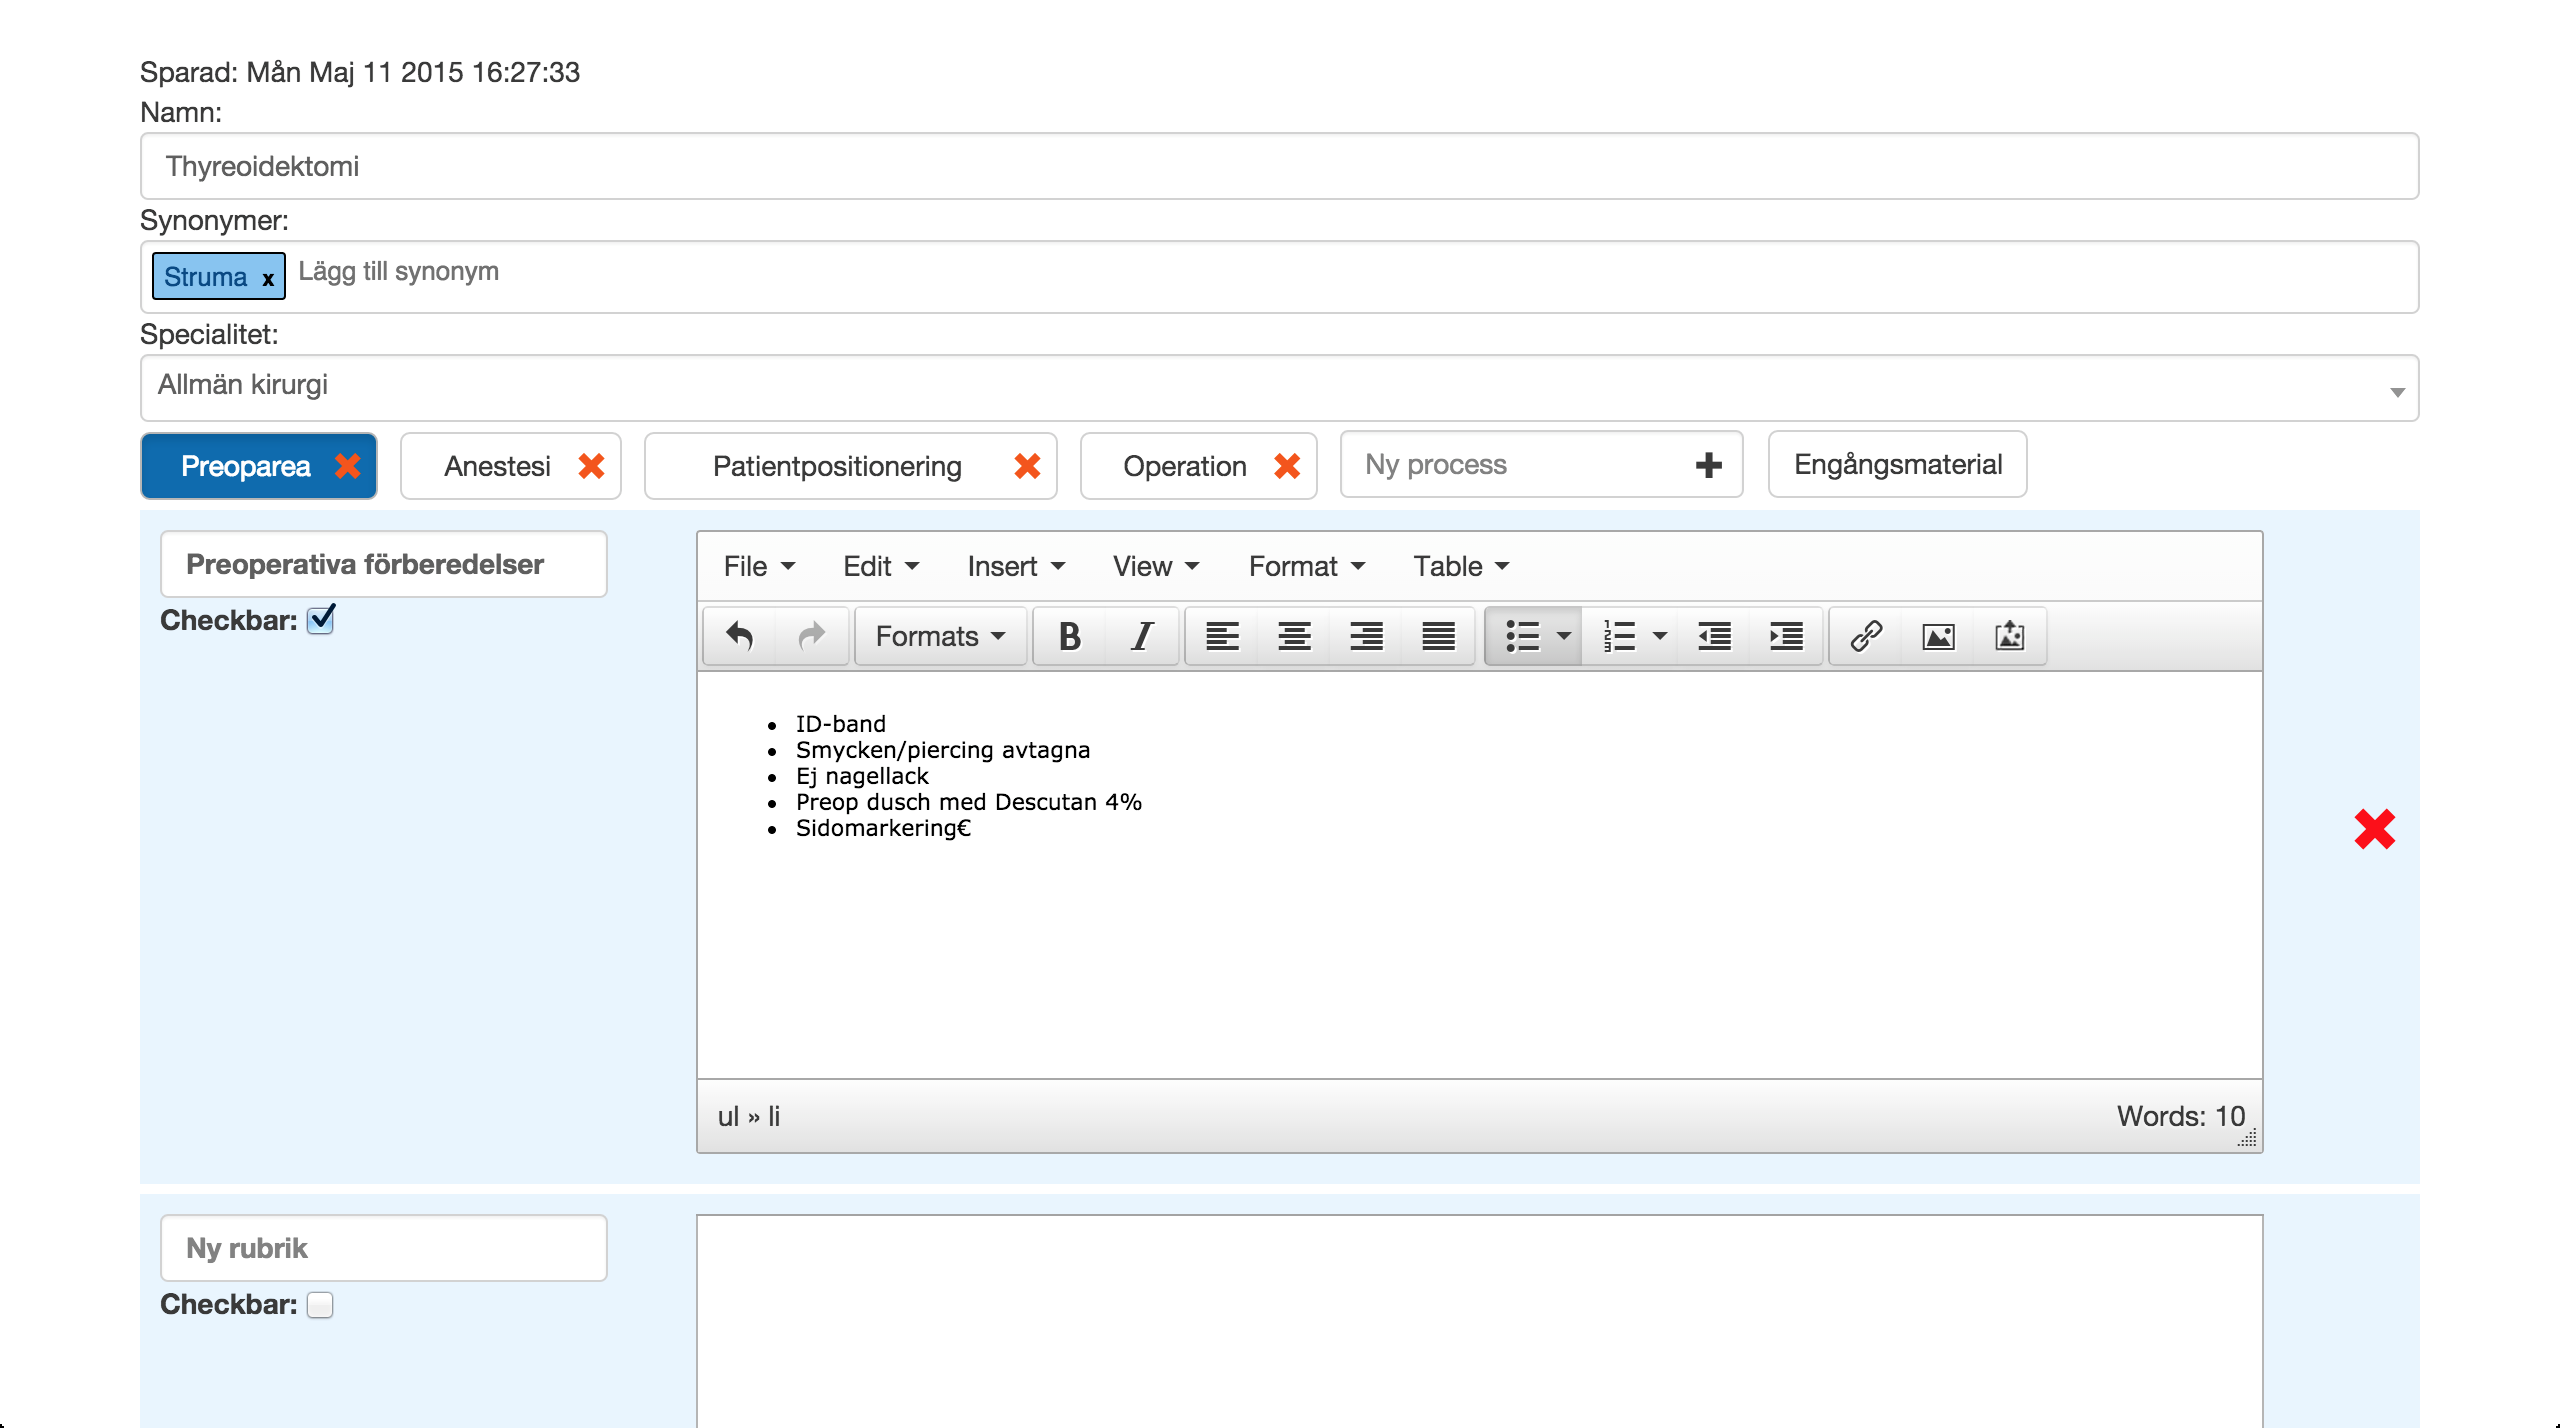
\includegraphics[width=0.9\textwidth]{images/site/handboksredigering}
  \caption{Redigering av plocklista för handbok}
  \label{fig:handboksredigering}
\end{figure}


I exemplet har underrubriken ''Preoperativa förberedelser'' lagts till under processteget ''Preopera''. Denna redigering använder sig av en wysiwyg-editor. Innehållet kan på så sätt formateras efter olika behov. I exemplet har innehållet strukturerats som en punktlista. 

I redigeringsvyn kan man utöver att redigera all information även sortera processer och rubriker genom att dra och släppa dem.

Under processteget engångsmaterial skapar man plocklistan. Ett exempel visas i figur \ref{fig:plocklistaredigering2}. Artiklar kan läggas till genom att söka på dem i kartoteket och antalet kan redigeras.

\begin{figure}[h!]
  \centering
  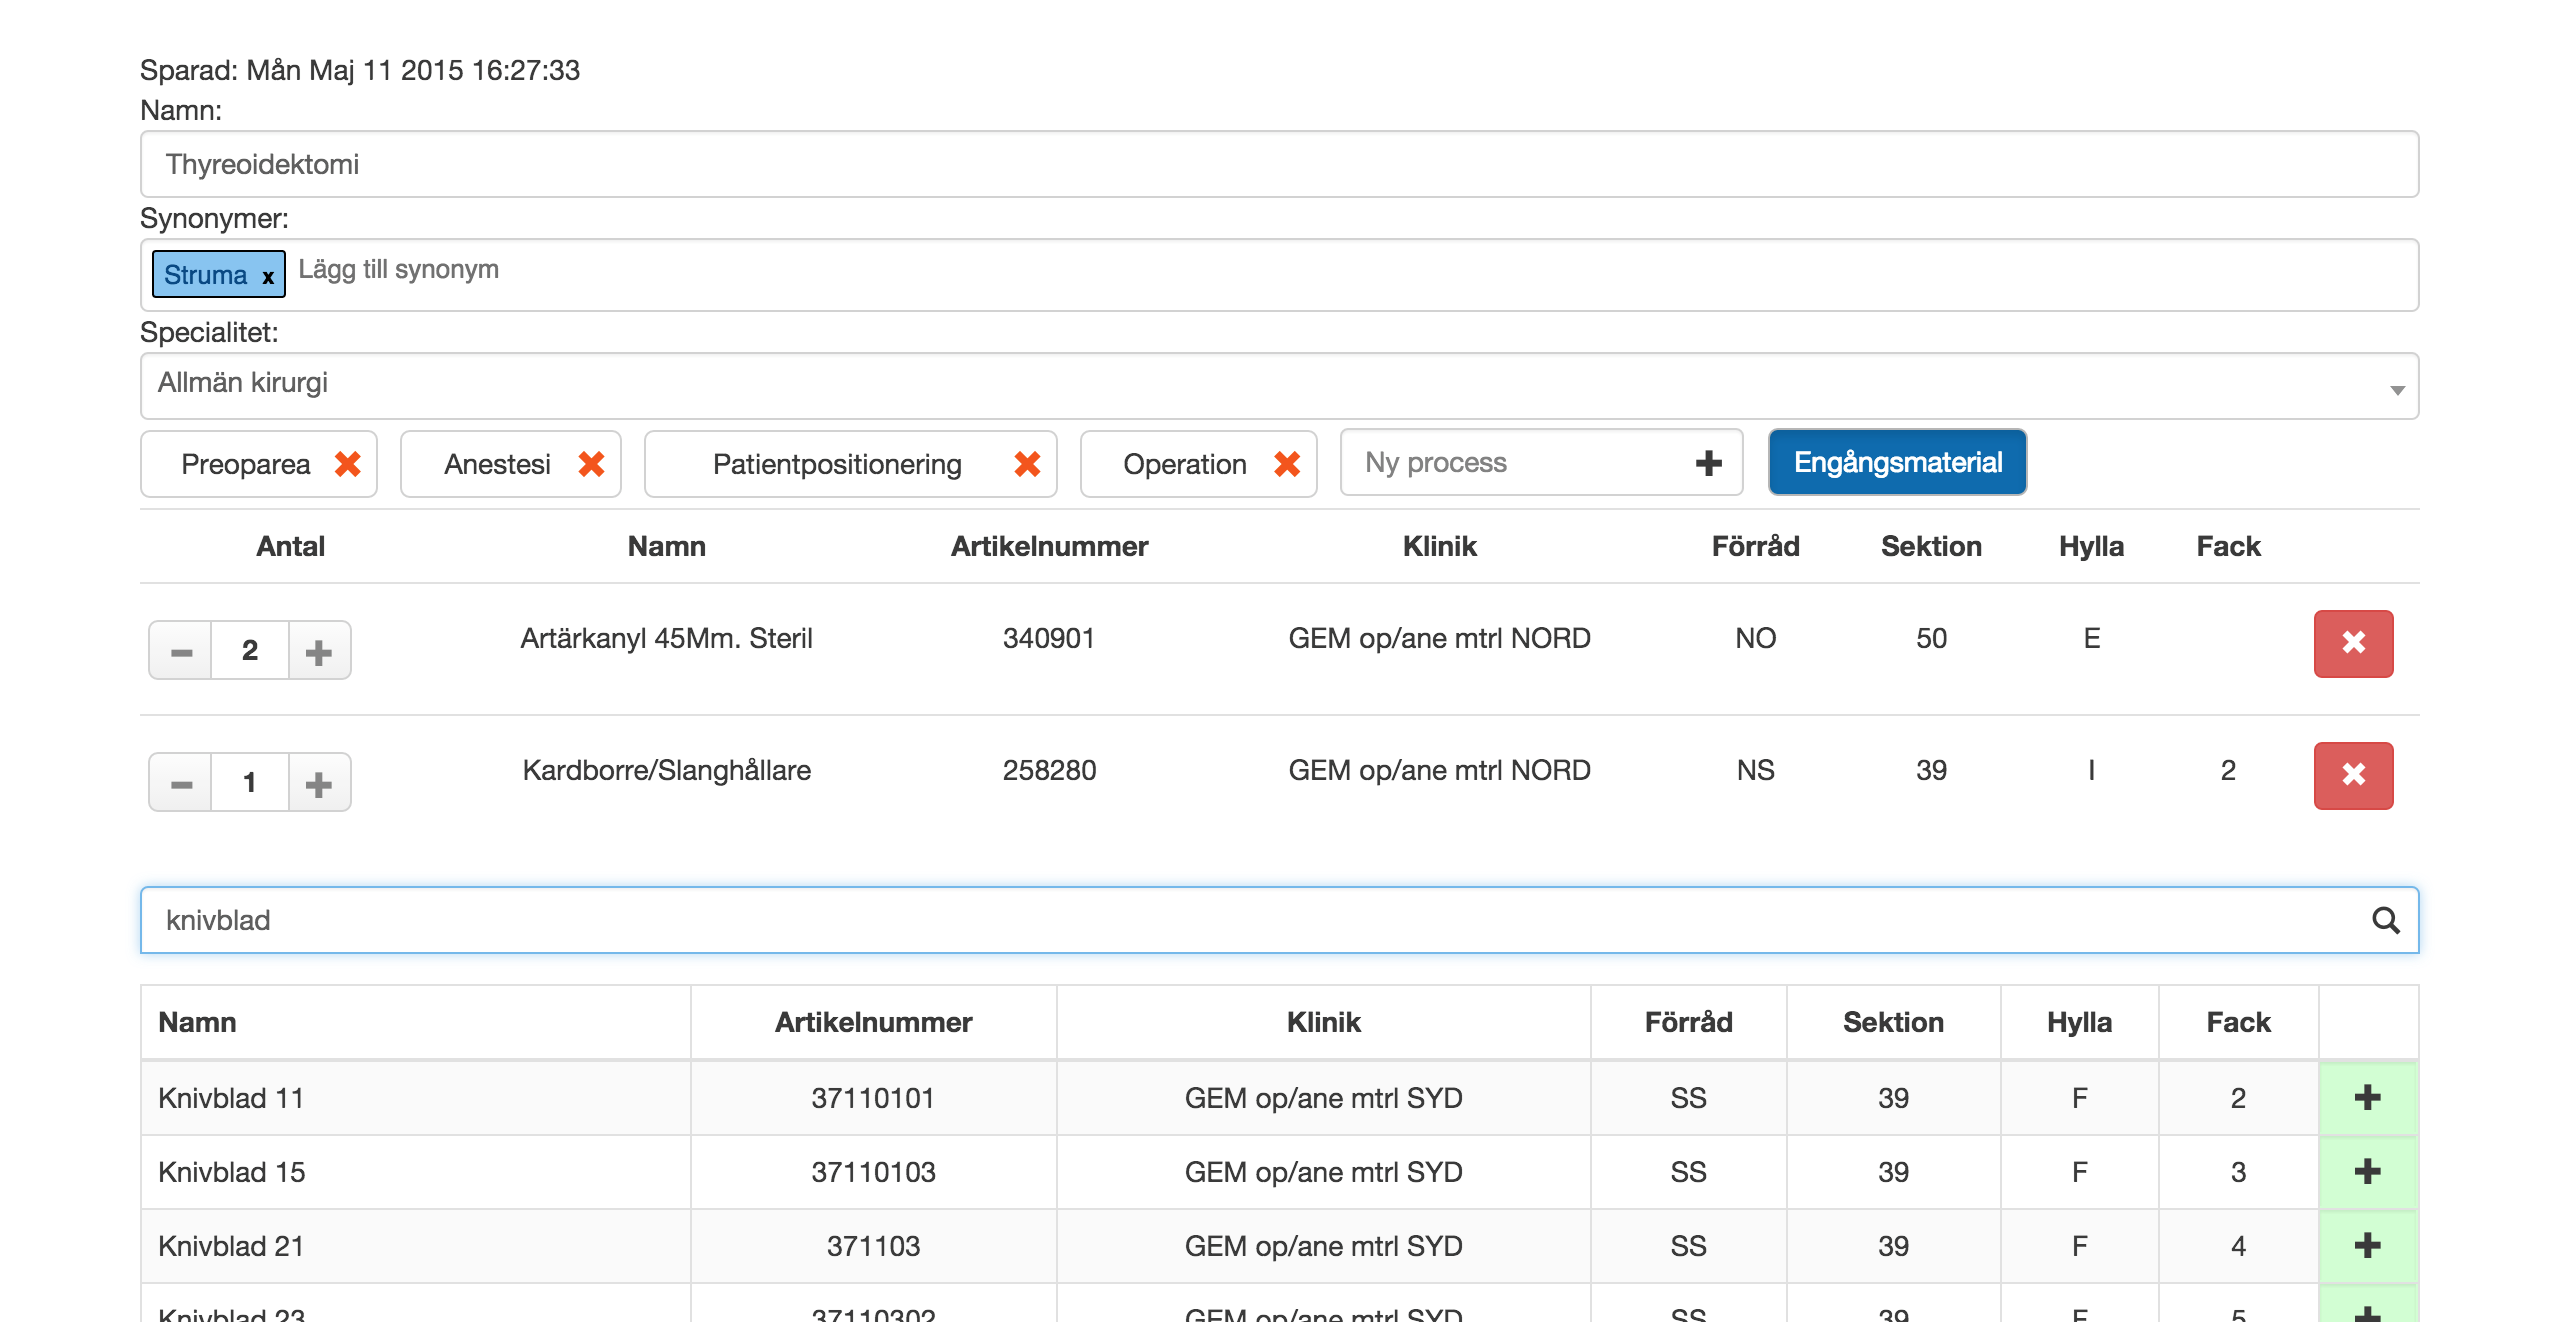
\includegraphics[width=0.9\textwidth]{images/site/plocklistaredigering2}
  \caption{Redigering av plocklista för handbok}
  \label{fig:plocklistaredigering2}
\end{figure}


Innan en redigerad eller ny handbok publiceras måste den granskas av en annan person. Detta görs genom att trycka på knappen skicka till granskning längst ned i redigeringsvyn.

\subsubsection{Operationsförberedelse}
En operationsförberedelse är en instans av en handbok vilket medför att att flera operationsförberedelser kan skapas från samma handbok. En operationsförberedelse ser nästan likadan ut som en handbok.
Det som skiljer sig är att vissa av rubrikerna för förberedelser och artiklar i plocklistan går att checka av när de är förberedda eller plockade.

\begin{figure}[h!]
  \centering
  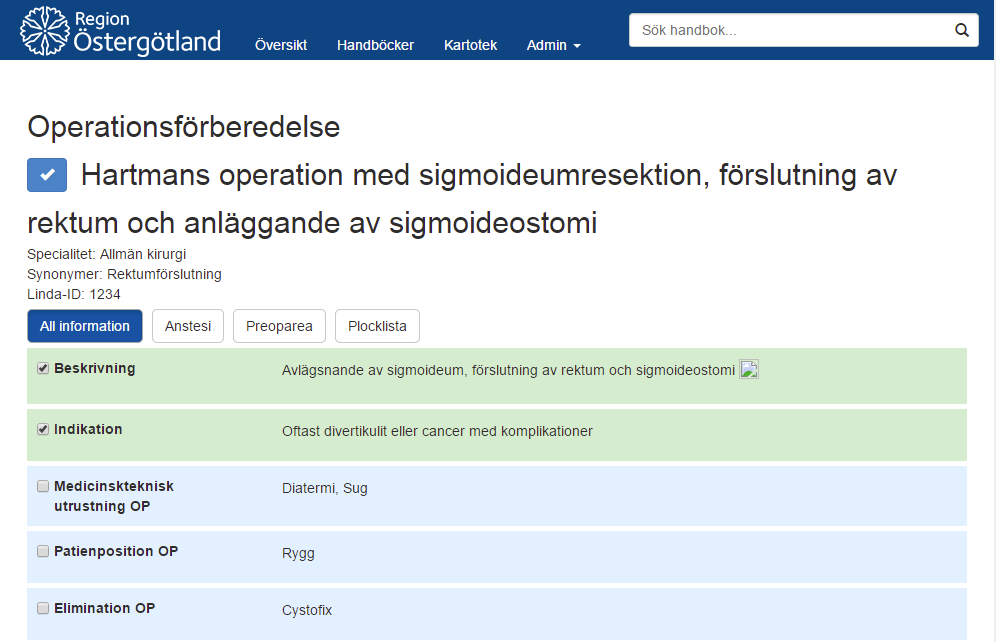
\includegraphics[width=0.9\textwidth]{images/site/op}
  \caption{Förberedelsevyn}
  \label{fig:op}
\end{figure}

I figur \ref{fig:op} kan man se att rubrikerna går att checka av när de är klara. Jämför med figur \ref{fig:handbok} där rubrikerna inte går att checka av. När operationen är klar kan en administratör ta bort operationsförberedelsen.
%Rent tekniskt så kan man se en operationsförberedelse som en instans av en handbok. Flera operationsförberedelser kan alltså vara skapade från samma handbok.
\subsubsection{Plocklista}
En operationsförberedelse har en plocklista med artiklar som behövs till operationen. Den ligger under fliken engångsmaterial.
Listan används för att hitta artiklar i lagret och för att checka av dem när de plockats. För att underlätta plockningen och göra den mer effektiv kan man välja att sortera artiklarna beroende på plockplats.

\begin{figure}[h!]
  \centering
  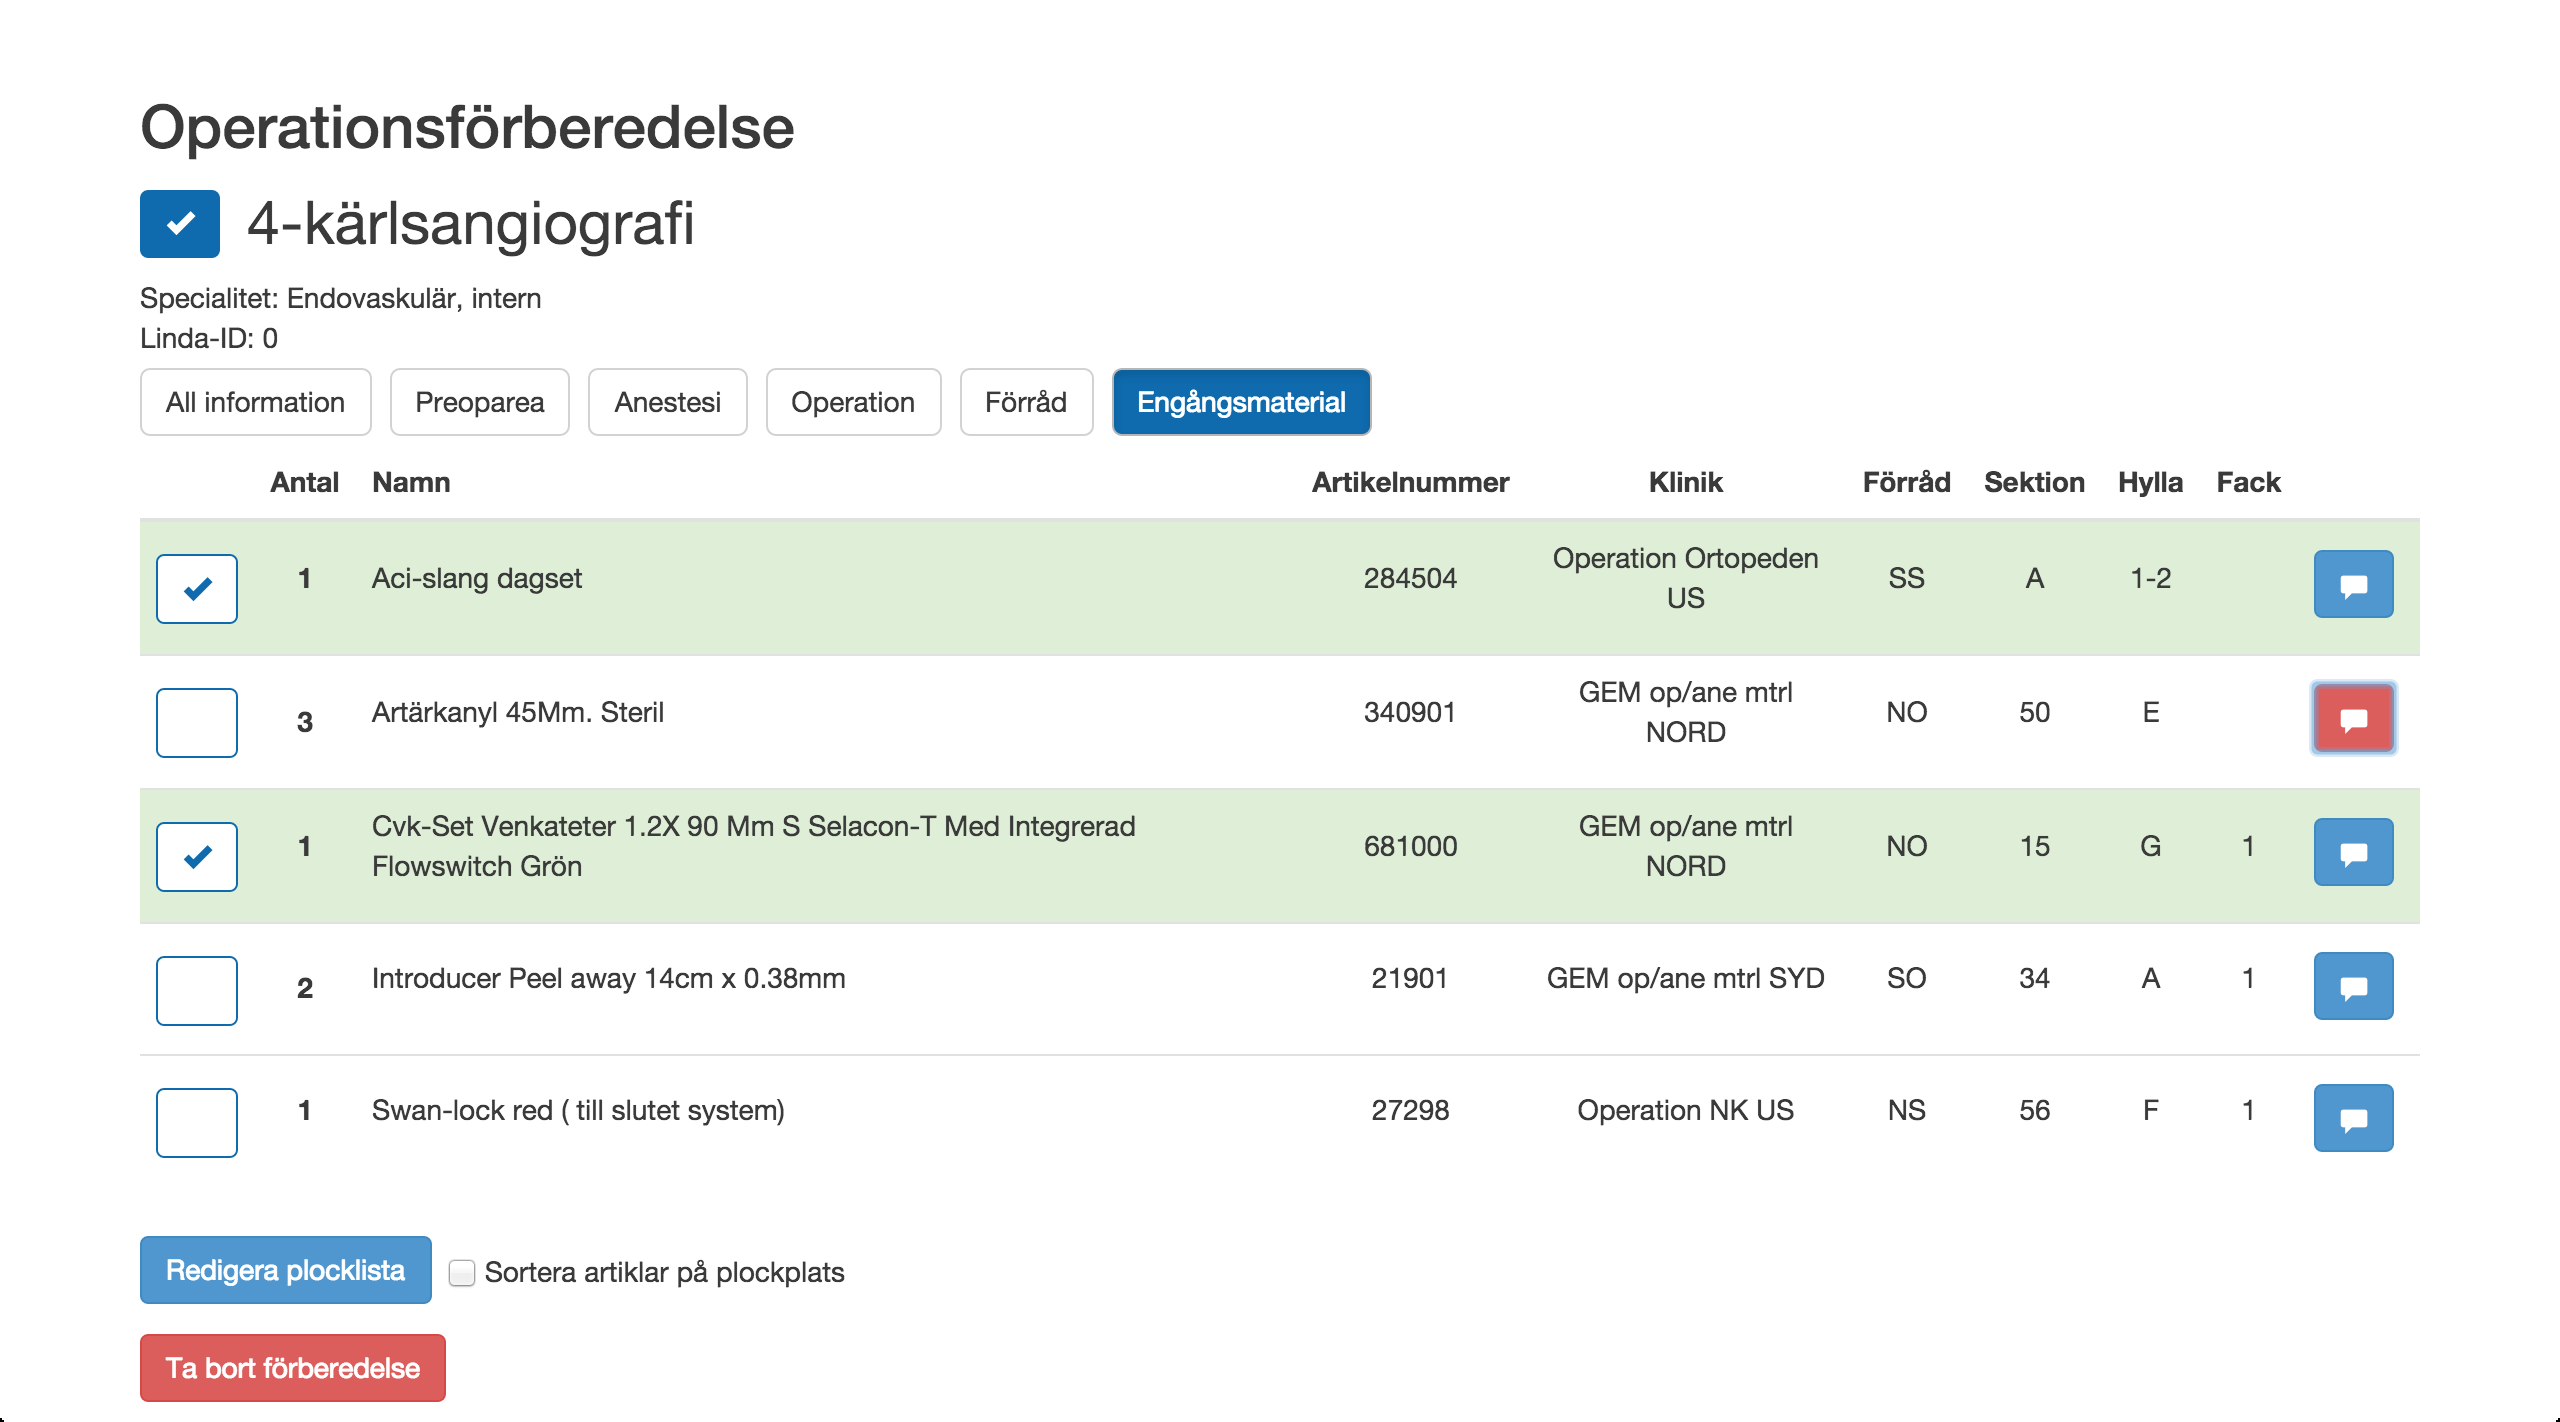
\includegraphics[width=0.9\textwidth]{images/site/plocklista}
  \caption{Plocklista}
  \label{fig:plocklista}
\end{figure}
I figur \ref{fig:plocklista} kan man även se att det finns stöd för att lägga en kommentar på en artikel.
Det är vanligt att en artikel är slut eller utbytt och man kan då lägga en kommentar på varför man inte kunde hämta den artikeln och även hur man har löst det istället. Ett exempel på kommentar visas i figur \ref{fig:kommentar}.

\begin{figure}[h!]
  \centering
  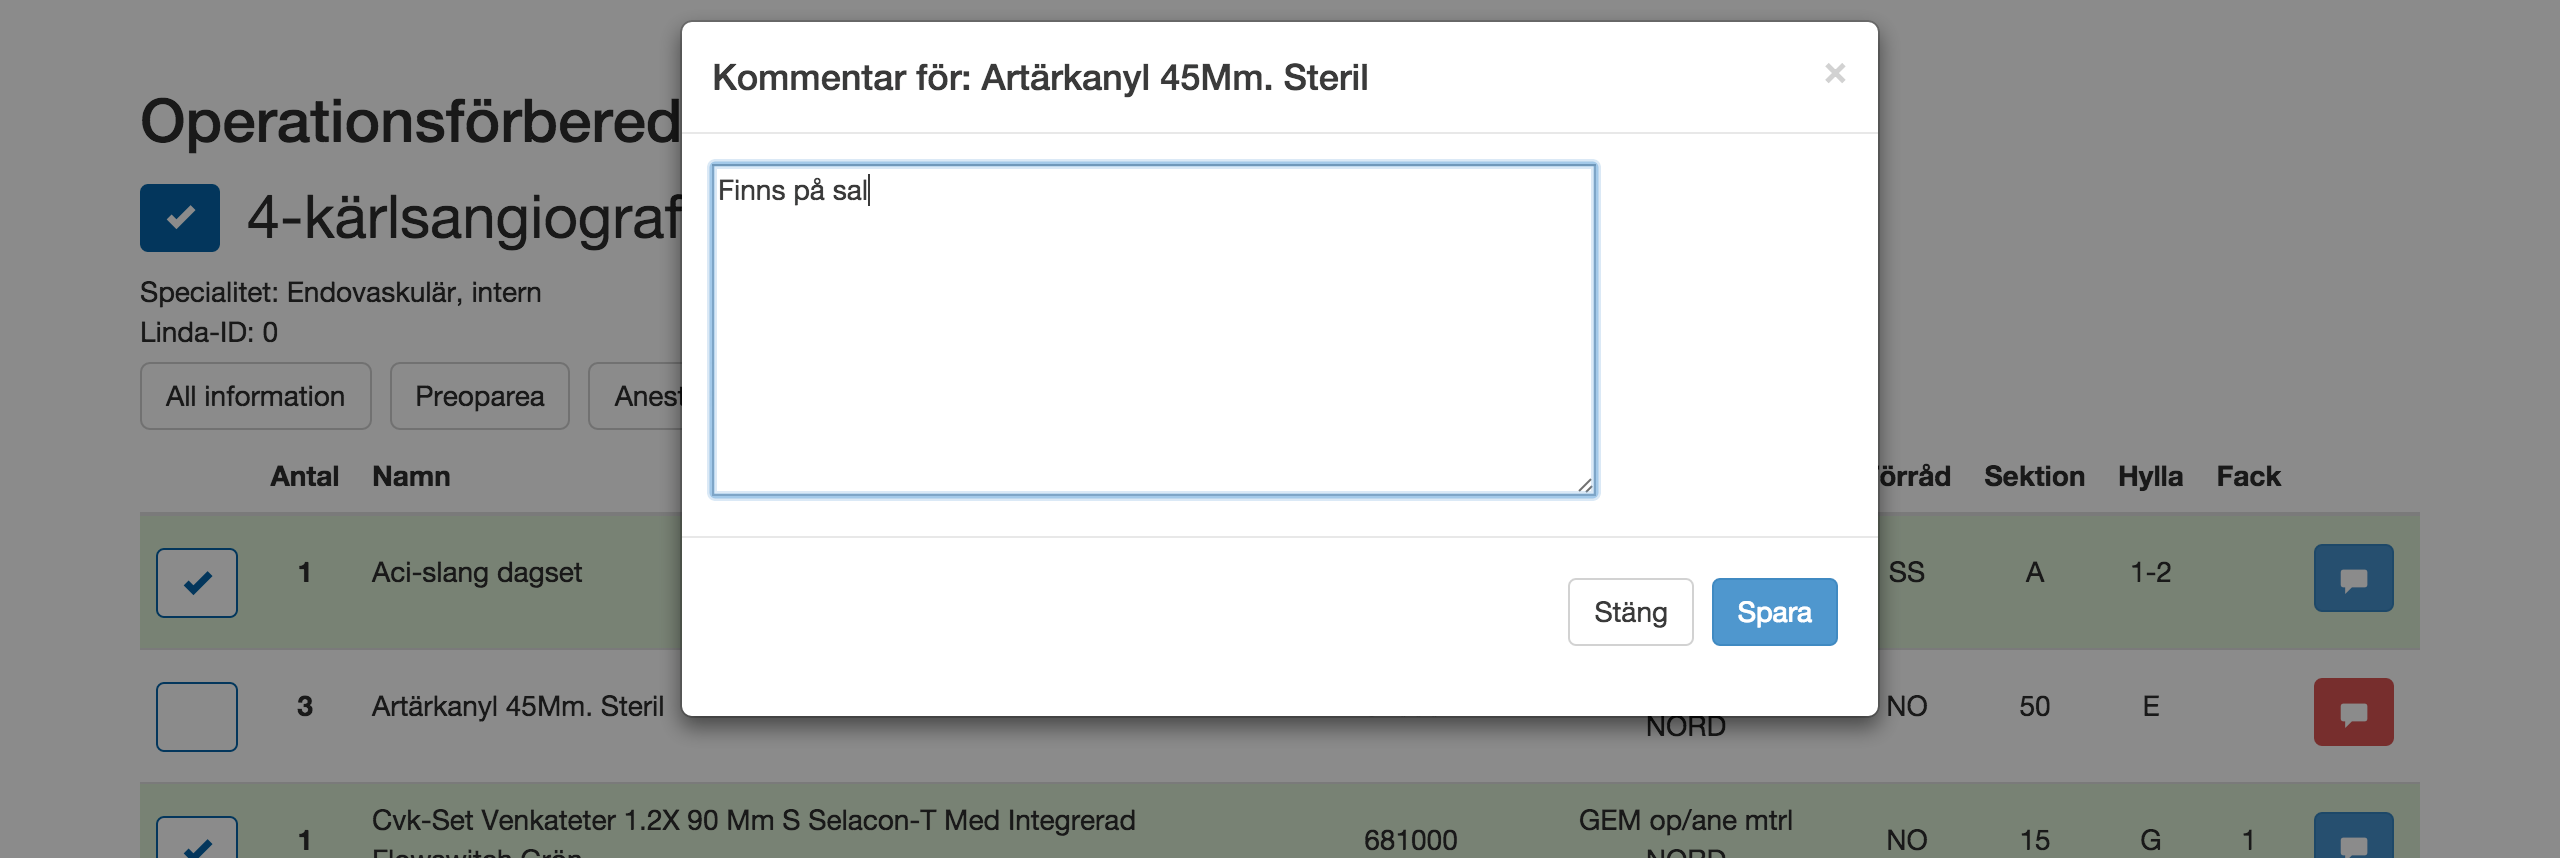
\includegraphics[width=0.9\textwidth]{images/site/kommentar}
  \caption{Kommentar}
  \label{fig:kommentar}
\end{figure}

Plocklistan kan under en pågående operation också redigeras. I figur \ref{fig:plocklistaredigering} visas hur man i redigeringsläget kan lägga till nya artiklar. Man kan i detta läge också ändra antalet för en specifik artikel eller välja att ta bort artiklar.

\begin{figure}[h!]
  \centering
  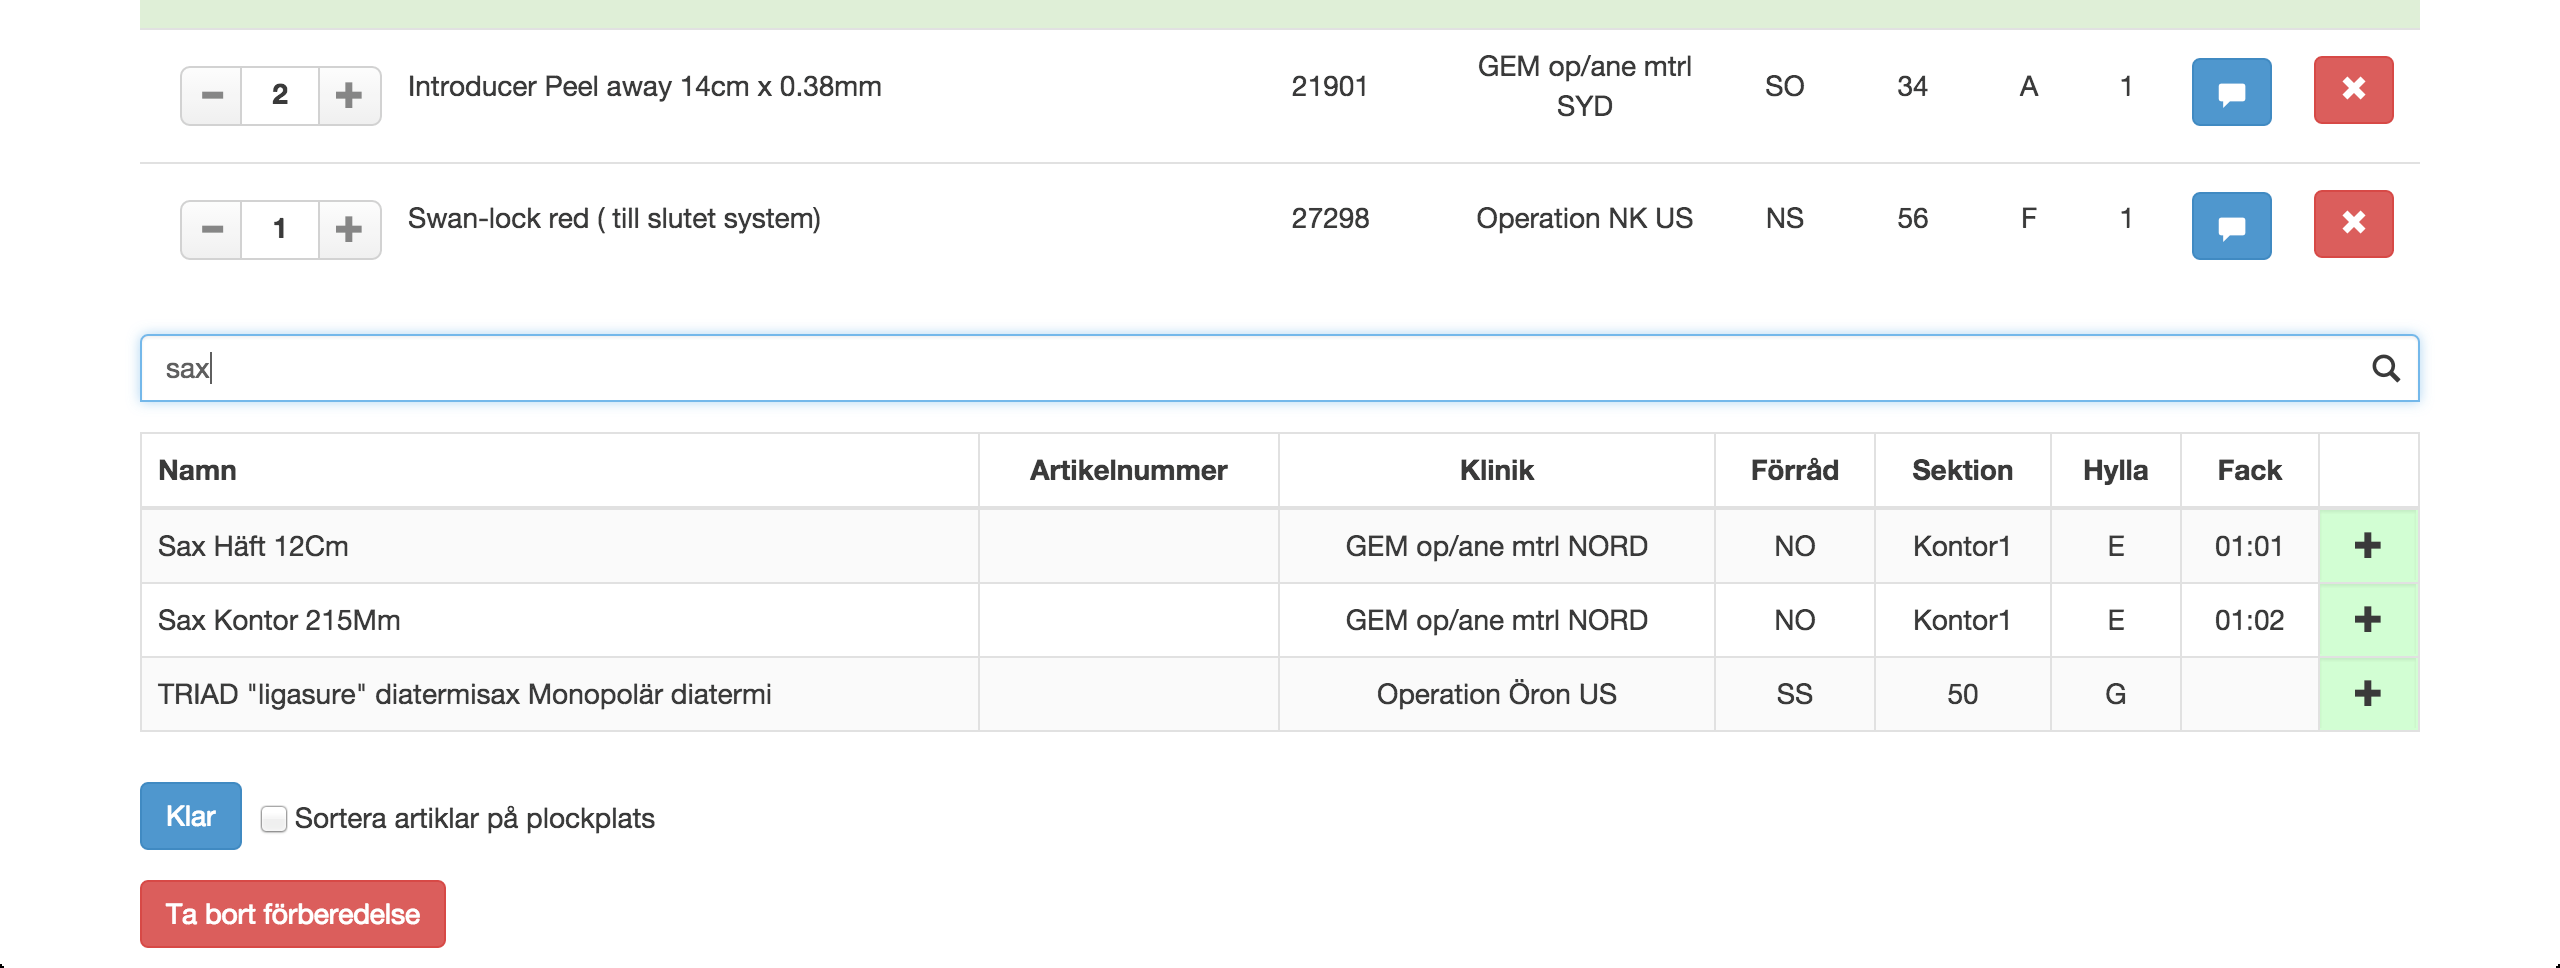
\includegraphics[width=0.9\textwidth]{images/site/plocklistaredigering}
  \caption{Redigering av plocklista för operationsförberedelse}
  \label{fig:plocklistaredigering}
\end{figure}

\subsubsection{Kartoteket}
Kartoteket är en artikeldatabas med allt engångsmaterial som används till operationer. I figur \ref{fig:kartoteket} visas hur kartoteket ser ut. 
\begin{figure}[h!]
  \centering
  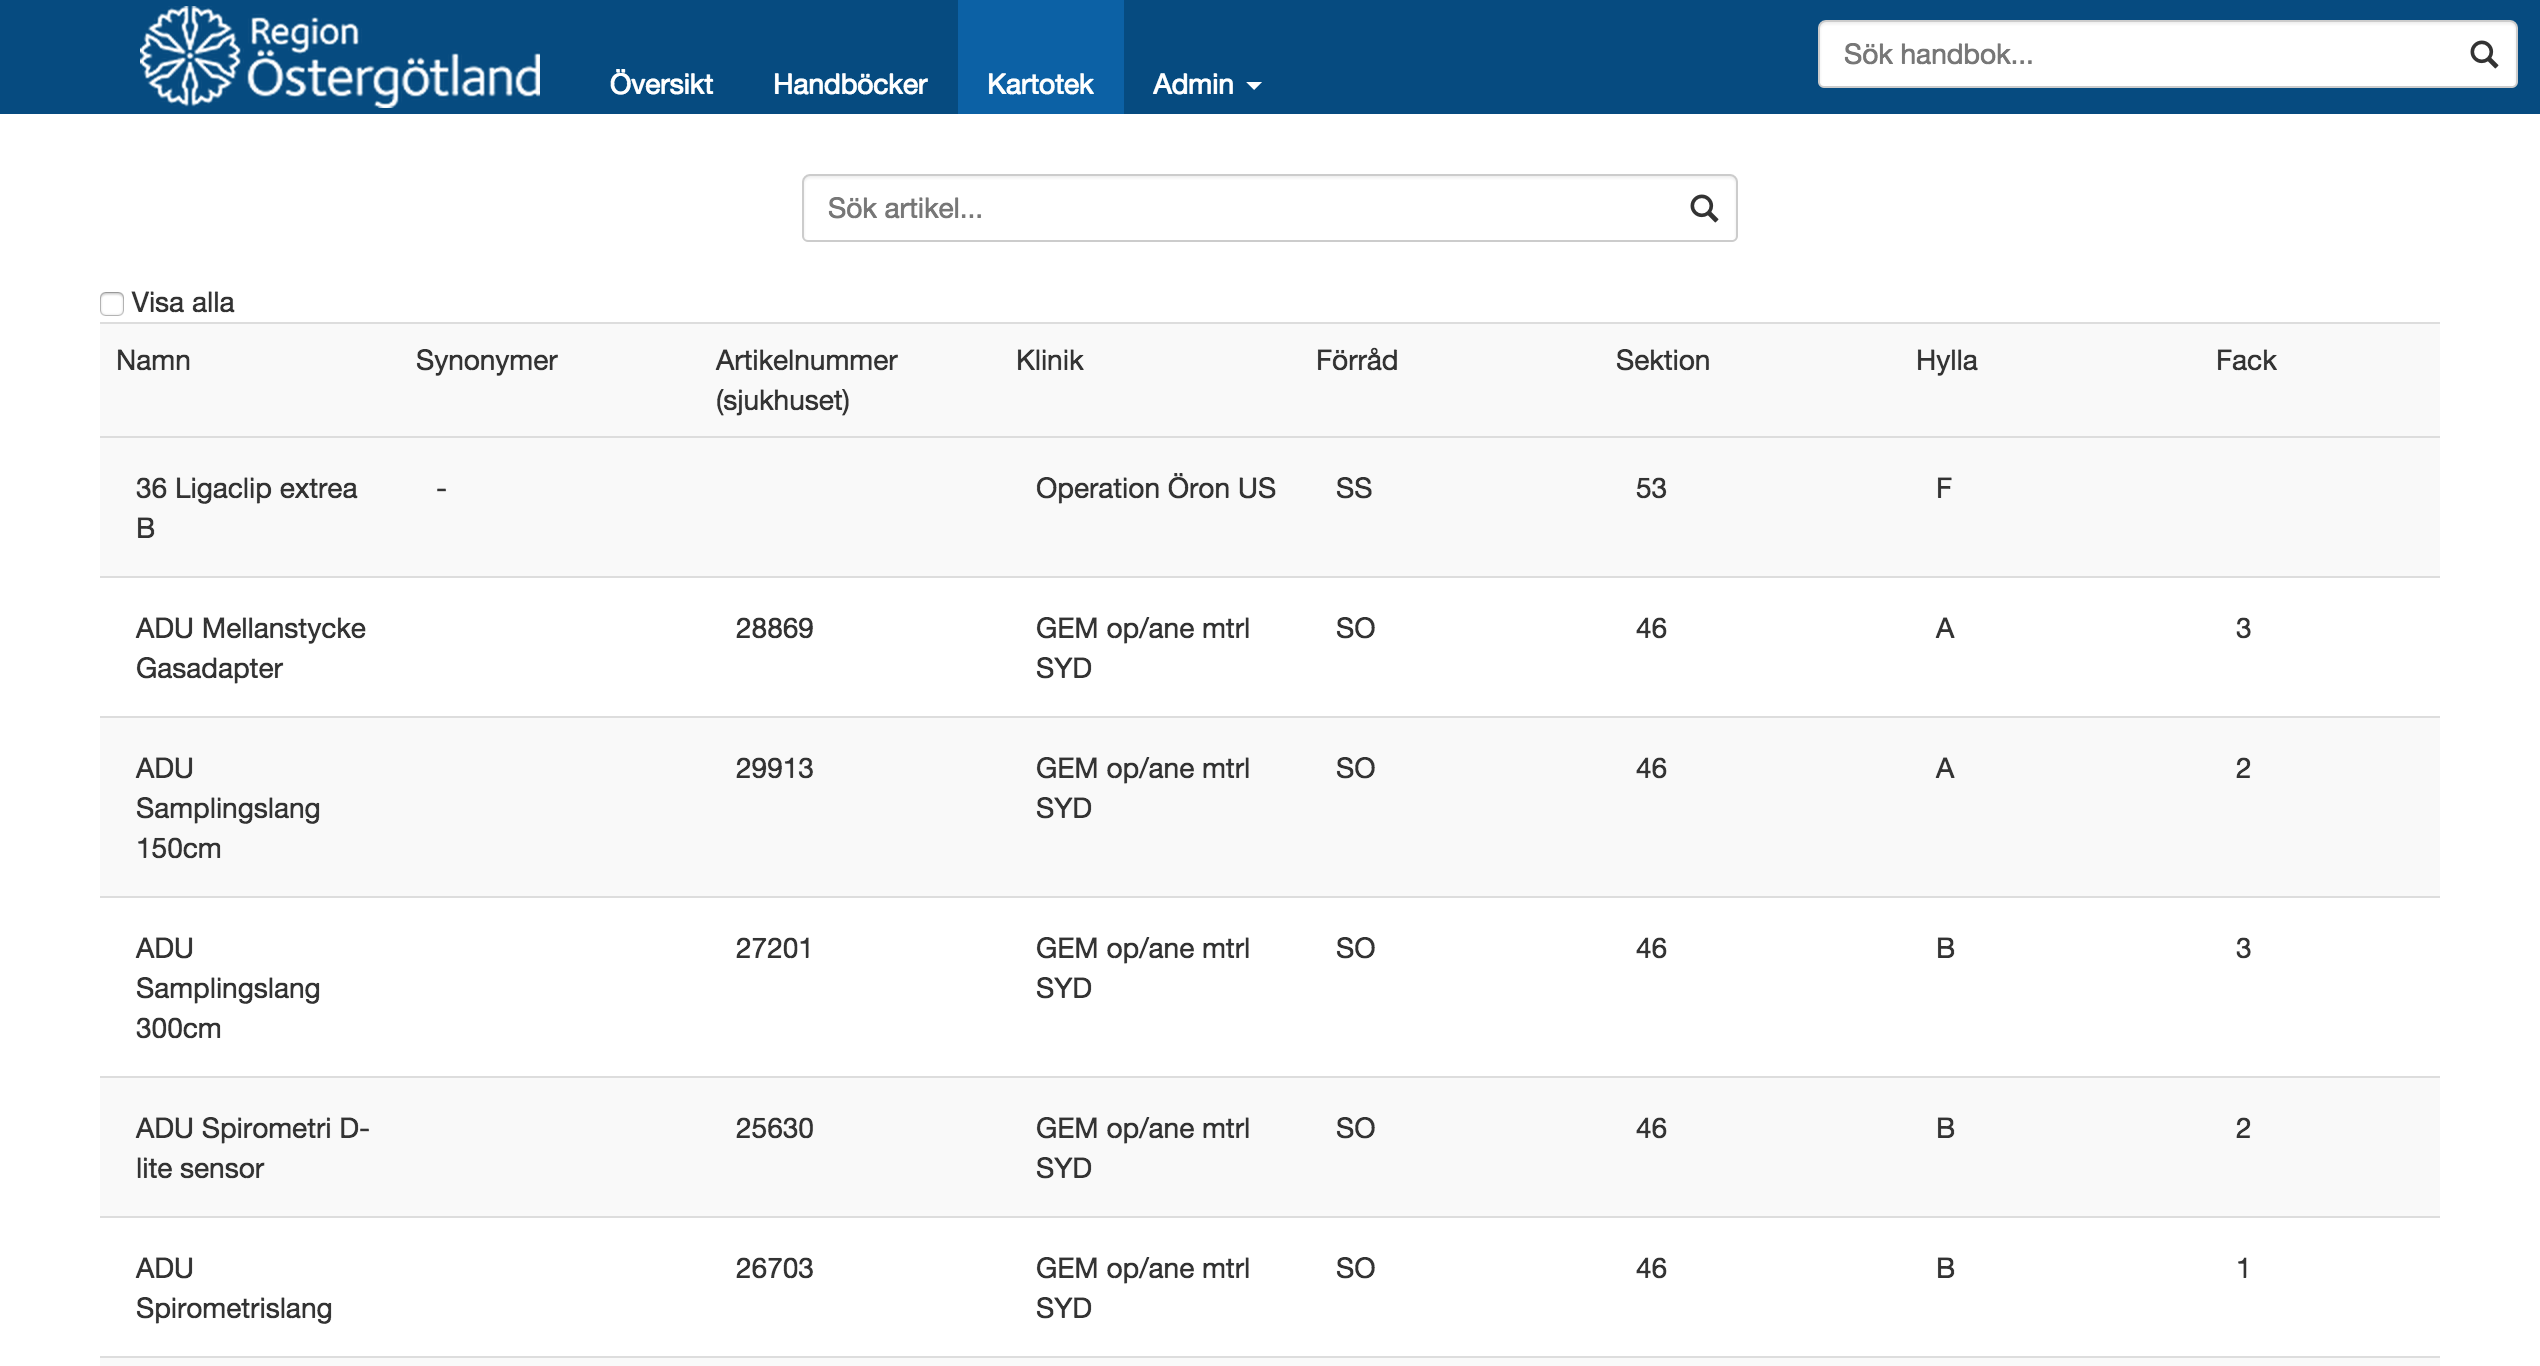
\includegraphics[width=0.9\textwidth]{../images/kartotek1.png}
  \caption{Kartoteket}
  \label{fig:kartoteket}
\end{figure}
Artiklarna är listade i en tabell och i kolumnerna visas information relaterad till artikeln. En vanlig användare kan se informationen som visas i figur\ref{fig:kartoteket}. För en administratör kan mer information visas såsom pris. En administratör kan också redigera och lägga till nya artiklar. Kartoteket diskuteras mer i djup i den enskilda utredningen A-Kartoteket.%Vet inte hur jag ska referera egentligen

%Lägg eventuellt till adminvyn och skriv om det.

\subsection{Utvecklingen}
Här nedan beskrivs resultatet av hur utvecklingen inom gruppen har fungerat,
och huruvida de olika hjälpmedlen har hjälpt eller stjälpt.

\subsubsection{SCRUM}
Utvecklingen i SCRUM-form har fungerat bra,
dock har utvecklingen som beskriven i metod inte varit i rent SCRUM-format utan har modifierats för att bättre passa gruppen.
Ett möte med handledare har hållits en gång i veckan där handledaren har haft möjlighet att ta upp saker som denne tyckt har behövts,
sedan har gruppen hållit ett kort SCRUM-möte där man fått förklara vad man gjort förra veckan och vad man planerat
att göra kommande vecka. Under mötets gång har man noterat om det är någonting som har behövt diskuteras
vidare och detta har då noterats, varpå gruppen har gått igenom dessa frågor efteråt. Detta har fungerat väldigt bra då man på detta sättet inte har fått några större avbrott och alla hela tiden kunna hålla fokus. Efter SCRUM-mötena så har ordet varit fritt och alla har haft möjligheten att komma med synpunkter eller åsikter över någonting.

\subsubsection{Samarbete i gruppen}
Samarbetet i gruppen har fungerat väldigt bra, kodstugorna som gruppen höll under förstudien var alla nöjda med, de som var mindre erfarna med webbprogrammering kände att de fick all den hjälp de behövde när de körde fast i sitt arbete och därför kändes det naturligt för hela gruppen att fortsätta med dessa även under utvecklingsfasen. 

Några av de rollspecifika uppgifter som genomfördes kan ses nedan.
\begin{itemize}
\item Arkitekten tog snabbt fram en arkitekturplan som sedan följdes genom hela projektet och fanns som stöd under utvecklingen för frågor om plattformen.
\item Kvalitetssamordnaren tog fram en kvalitetsplan.
\item Dokumentansvarige kollade så dokumenten följde dokumentstandarden som var definerad i kvalitetsplanen följdes och informerade om ett system för referenser.
\item Teamledaren skrev en projektplan, skickade in tidrapportering och planerade när arbetet skulle ske.
\item Testledaren skrev en testplan och en testrapport. I början skedde inte mycket testning, men i mitten av iteration 2 så började det testas mer. Testledaren var då den person som gjorde alla automatiserade tester.
\item Utvecklingsledaren tog i början fram exempel på verktyg och en användarmanual för den föreslagna utvecklingsmiljön.  
\item Analysansvarige skötte all kundkontakt under hela projektet och tog fram en kravspecifikation. 
\end{itemize}   

%\subsection{Gruppens gemensamma erfarenheter}
%\subsection{Översikt över de inviduella utredningarna}
